% This file was created with tikzplotlib v0.10.1.
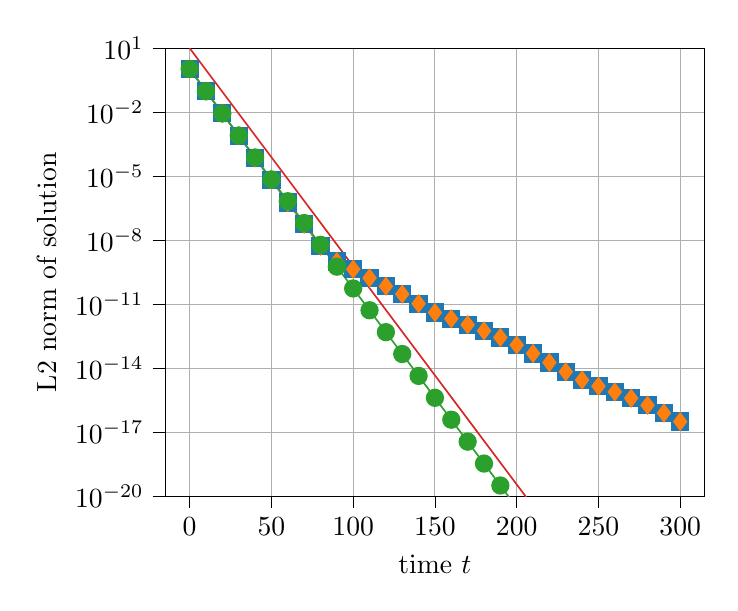
\begin{tikzpicture}

\definecolor{crimson2143940}{RGB}{214,39,40}
\definecolor{darkgray176}{RGB}{176,176,176}
\definecolor{darkorange25512714}{RGB}{255,127,14}
\definecolor{forestgreen4416044}{RGB}{44,160,44}
\definecolor{steelblue31119180}{RGB}{31,119,180}

\begin{axis}[
log basis y={10},
tick align=outside,
tick pos=left,
x grid style={darkgray176},
xlabel={time $t$},
xmajorgrids,
xmin=-15, xmax=315,
xtick style={color=black},
y grid style={darkgray176},
ylabel={L2 norm of solution},
ymajorgrids,
ymin=1e-20, ymax=10,
ymode=log,
ytick style={color=black},
ytick={1e-23,1e-20,1e-17,1e-14,1e-11,1e-08,1e-05,0.01,10,10000},
yticklabels={
  $\mathdefault{10^{-23}}$,
  $\mathdefault{10^{-20}}$,
  $\mathdefault{10^{-17}}$,
  $\mathdefault{10^{-14}}$,
  $\mathdefault{10^{-11}}$,
  $\mathdefault{10^{-8}}$,
  $\mathdefault{10^{-5}}$,
  $\mathdefault{10^{-2}}$,
  $\mathdefault{10^{1}}$,
  $\mathdefault{10^{4}}$
}
]
\addplot [semithick, steelblue31119180, mark=square*, mark size=3, mark options={solid}]
table {%
0 1.05962445391129
10 0.0993374798741873
20 0.00885139563395991
30 0.000797636495806965
40 7.13649011310969e-05
50 6.62140449455375e-06
60 5.96660036962194e-07
70 5.73361702198827e-08
80 5.4697065574544e-09
90 1.01403848450589e-09
100 4.41006819709737e-10
110 1.71841756962258e-10
120 7.05351070816565e-11
130 3.0156130005597e-11
140 1.07482980809563e-11
150 4.13735828815523e-12
160 2.11223417534529e-12
170 1.11120879493413e-12
180 5.74128248578687e-13
190 2.81074858026958e-13
200 1.24902634998799e-13
210 4.97891246401207e-14
220 1.86805530660425e-14
230 6.91456579694307e-15
240 2.84955129692088e-15
250 1.46122746302131e-15
260 7.88643182437221e-16
270 4.00143292010953e-16
280 1.87818291559133e-16
290 8.11654694953298e-17
300 3.21586712463098e-17
};
\addplot [semithick, darkorange25512714, mark=diamond*, mark size=3, mark options={solid}]
table {%
0 1.05962445391129
10 0.0983988836955729
20 0.00876395264136963
30 0.000796196581500739
40 7.17833020901883e-05
50 6.64321717963424e-06
60 5.9031917862261e-07
70 5.56823040474351e-08
80 5.29791340654292e-09
90 1.00550938831331e-09
100 4.41040462899321e-10
110 1.71885230219556e-10
120 7.05376022238178e-11
130 3.0158313814246e-11
140 1.07490361784002e-11
150 4.13762684041183e-12
160 2.11239509583167e-12
170 1.11126357104592e-12
180 5.74135733948613e-13
190 2.81077708367403e-13
200 1.24905815107576e-13
210 4.97902008459404e-14
220 1.86807877259329e-14
230 6.91469025557143e-15
240 2.84962166691169e-15
250 1.46125197015362e-15
260 7.88651272353789e-16
270 4.0014544496596e-16
280 1.87818892354193e-16
290 8.11657788318577e-17
300 3.21588454553612e-17
};
\addplot [semithick, forestgreen4416044, mark=*, mark size=3, mark options={solid}]
table {%
0 1.05962445391129
10 0.0955215283164192
20 0.00872709845052959
30 0.000807483575033667
40 7.55224354166436e-05
50 7.12194362312964e-06
60 6.75381493260096e-07
70 6.42523358471142e-08
80 6.12035423254634e-09
90 5.82890438104887e-10
100 5.54487864022824e-11
110 5.26535874460931e-12
120 4.98954910374828e-13
130 4.71803473666431e-14
140 4.45222983557405e-15
150 4.19397393935627e-16
160 3.94523533294454e-17
170 3.70788972324616e-18
180 3.48355228799717e-19
190 3.27345083944987e-20
200 3.07833599884726e-21
210 2.89843007022948e-22
220 2.73341889503217e-23
230 2.58248981685172e-24
240 2.44441425223163e-25
250 2.31766668312186e-26
260 2.20056553025092e-27
270 2.09141772320652e-28
280 1.98864915399293e-29
290 1.89090724718026e-30
300 1.79712797747339e-31
};
\addplot [semithick, crimson2143940]
table {%
0 10
10 0.951111830888997
20 0.090461371485702
30 0.00860388806584957
40 0.000818325973107418
50 7.78319514546217e-05
60 7.40268898496687e-06
70 7.04078507399366e-07
80 6.69657398262203e-08
90 6.36919074129526e-09
100 6.05781266723458e-10
110 5.76165729711604e-11
120 5.47998042081499e-12
130 5.2120742112772e-13
140 4.95726544581719e-14
150 4.71491381437395e-15
160 4.48441031047303e-16
170 4.2651757008515e-17
180 4.05665906990013e-18
190 3.85833643526517e-19
200 3.66970943113078e-20
210 3.49030405587341e-21
220 3.31966948094105e-22
230 3.15737691796417e-23
240 3.00301854125156e-24
250 2.85620646296337e-25
260 2.71657175838608e-26
270 2.58376353885993e-27
280 2.45744807002931e-28
290 2.3373079332002e-29
300 2.22304122769743e-30
};
\end{axis}

\end{tikzpicture}
